\TUchapter{Discrete Extensions}
\TUsection{Introduction}
For various reasons, the adaptation of the attack graph formalism described in
the preceding chapter for hybrid purposes depends upon the addition of a number
of entirely discrete elements. Their inclusion produces a transitional
attack graph formalism that is not yet appropriate for hybrid modeling but that
contains a number of enhancements suitable for discrete system modeling.

This chapter introduces these enhancements, which include a working lexicon of
standard terms for topologies and qualities based upon the Common Vulnerability
Enumeration and National Vulnerability Database; some syntactic
changes to ease the modeling of information systems; a scheme for integrating with
the Common Platform Enumeration~\cite{buttner2009common}.

\TUsection{Working Lexicon}
\TUsubsection{Introduction}
Because of the unrestricted nature of the terms available to a modeler
in this version of the attack graph framework, in order to proceed systematically
some conventions must be established in the use of terms. This thesis recommends
a set of conventions designed to ease the goal of automated exploit pattern extraction
from the National Vulnerability Database (NVD) maintained by the 
National Institute of Standards and Technology (NIST), which among other roles
indexes MITRE's Common Vulnerability Enumeration (CVE). ``NVD includes 
databases of security checklists, security related software flaws, 
misconfigurations, product names, and impact metrics''~\cite{nvdhome}.
\TUsubsection{National Vulnerability Database}
Several concepts are used across the NVD's index of vulnerabilities; they
strongly inform the working lexicon employed in this thesis and include
a vulnerability's access vector and impact type.
\TUsubsubsection{Access vector}
The access vector of a vulnerability on NVD refers to the logical location from
which the attacker may launch the attack. The possible attack vectors according
to the National Vulnerability Database are as follows.
\begin{description}
\item[Local] The vulnerability is exploitable through physical or local account access
    to the device on which the vulnerability resides.
\item[Adjacent Network] The vulnerability is exploitable through access to a network
    that is adjacent to the vulnerable host; that is, the attacker must be in the same
    broadcast domain or collision domain (e.g. the same network segment or VLAN).
\item[Network] No local or adjacent access is required to exploit the vulnerability;
    in other words, it is exploitable over the Internet.
\end{description}
\TUsubsubsection{Impact Type}
The vulnerability's impact type on NVD places the effects of the vulnerability's
exploitation on the target into one of the following categories, which 
correspond neatly with Microsoft's STRIDE framework. % CITE
\begin{description}
\item[Confidentiality] Confidentiality impacts allow the unauthorized disclosure 
    of information (corresponding to STRIDE's ``information disclosure'')
\item[Integrity] Allows modification of data (corresponding to STRIDE's ``tampering'')
\item[Availability] Availability impacts correspond to disruptions of service (STRIDE's
    ``denial of service'')
\item[Security Protection] The security protection category refers to the effects
    of exploits that provide unauthorized access to the target. This may be either
    general system access or application access. The security protection category
    corresponds roughly to STRIDE's ``elevation of privileges'' and also partly encompasses
    ``spoofing identity''. It has three subcategories:
    \begin{description}
    \item[User access] This subcategory refers to the attacker's gaining user level access
        to the operating system.
    \item[Administrative access] This subcategory refers to the attacker's gaining root level
        access to the operating system.
    \item[Other access] This subcategory refers to any other type of privileged access on
        the target.
    \end{description}
\end{description}
\TUsubsection{Topologies}
Introduction of actual terms begins with topologies, but first a note about the modeling
of adversaries is needed. 

Two approaches are possible for modeling the attacker. The first
is to design the network model so that it is, in a way, from the attacker's perspective.
In this scheme, henceforth the \emph{first person} strategy, the attacker is treated as
implicit, and its access and connections are considered properties of the system itself.
The adversary's access level to a server, for instance, would be modeled as a quality of
that server asset.

In the second approach, henceforth the \emph{third person} strategy, the attacker is
modeled as a first class part of the system: as an asset. Its properties, connections,
and access levels are modeled as qualities and topologies of the adversary asset.
This strategy, which is the one employed primarily in this thesis, can model multiple
adversaries. Aside from that difference, they are roughly equivalent and a matter
of taste on behalf of the modeler and analyst. This section's terminology, however,
assumes the third person model.

Two types of topology terms are introduced in this section: connection and access. These
correspond directly to the two NVD concepts introduced in the previous section.
\TUsubsubsection{Connection Topologies}
Connection topologies refer to how two assets are connected, over the network or otherwise.
They may be local, adjacent, or network connected. These connection topologies begin with
the word \texttt{connected}, followed by an underscore, then one of the three connection
types: \texttt{local}, \texttt{adjacent}, or \texttt{network}. For local and adjacent
connections, this is all that is necessary. 

For network connections it is
necessary to specify the available protocols individually. These are done by appending another
underscore, then the lower case version of the standard abbreviation for the protocol
(e.g. \texttt{connected\_network\_http} for web or \texttt{connected\_network\_ssh} for
secure shell).

Connections are one-way: the source of the connection topology is considered to be the
``client'' in the relationship, and the destination of the connection is considered
the ``server'', where such distinctions are meaningful.
\TUsubsubsection{Access Topologies}
Access topologies refer to trust relationships and distinguish what kind of access one
asset (possibly a program, individual, attacker, user, or other security principal) has
to another. Much like the subcategories of the Security Protection impact type,
there are three basic types of access topology (plus the lack of a topology, which
signifies a lack of any noteworthy trust or access relationship): user access,
root access, and other access.

They are named using the word \texttt{access}, followed by an underscore, followed
by the lowercase name of the access type, then, if the access type is \texttt{other},
an optional underscore delimited description of the access type (perhaps the name
of the application whose access level is in question). Examples include
\texttt{access\_user}, \texttt{access\_root}, \texttt{access\_other\_apache}, or
\texttt{access\_other\_vsftpd}.
\TUsubsection{Qualities}
Although qualities are used in a more \emph{ad hoc} fashion to describe entity-specific
asset properties, there is still a role for a standard quality structure in the
lexicon, namely a simple ``status'' type of property to be used in determining
whether an asset is enabled or disabled.
\TUsubsubsection{Status}
The status property is simple but powerful. Each asset that represents a host has a
quality named \texttt{status}. It may take the value \texttt{up} or \texttt{down}.
This allows exploits against or involving the host in question to require that it
be online as a precondition, and it provides a simple mechanism of action for
denial of service attacks to be modeled -- they simply have the postcondition of
a \texttt{status = down} quality fact.

\TUsection{Syntactic Sugar}
\TUsubsection{Directional Topologies}
This section introduces a new notation for specification of topologies. As it
is common to model bidirectional topologies, an additional convenience syntax
is now permitted to specify the directionality of a topology. As before, 
topologies are specified by the word~\texttt{topology}, followed by a colon, 
followed by the names of the assets in question; however, in the new syntax,
they are separated not by a comma but by a directionality symbol:~\texttt{->} to 
represent a one-way topology from the left asset to the right asset,
or~\texttt{<->} to represent a two-way topology. To promote readability, there
is no~\texttt{<-} directionality permitted.

Furthermore, the model has no innate distinction between one-way and two-way
topologies except the \texttt{<->} shorthand for specifying symmetric topologies.
That is to say, a bidirectional topology fact is actually implemented as
two unidirectional topology facts. Therefore, for example, if a bidirectional
topology exists in the fact base, one of its component directional topologies may
be removed by the realization of an exploit without affecting its reverse.
\TUsubsection{Value Assignment}
In preparation for the introduction of real-valued facts, the existing discrete
type of qualities, henceforth called ``token valued'', are given a special
assignment operator. Simply put, token values are assigned with the~\texttt{=}
operator and tested with the~\texttt{=} and~\texttt{!=} operators. This
enables a robust distinction between assignment operators and relational
operators.

Additionally, \texttt{delete} operations in postconditions take only a quality
name, with no value required (eliminating the confusing possibility of a
command to \texttt{delete quality:a,q!=5}, one of several deletion commands
that has little meaning).
\TUsubsection{Host Declaration and Status Proprocessing}
To support the use of status properties of host assets, a set of shorthand
syntax is now provided for denoting which assets represent hosts. In practice,
this has been observed to be the majority of modeled assets, so the shorthand
is highly convenient for modelers. Host denotation and status processing is 
done in two places: in the declaration of assets, and in the parameter list of 
exploits.

In the asset list declaration, up hosts are denoted by prefixing their name with
the symbol~\texttt{@}, a signal to the host preprocessor to automatically add
the \texttt{quality:hostname,status=up} fact; and down hosts are denoted with
the~\texttt{!@} symbol, automatically adding the down host quality fact.

Similarly, in exploit parameter lists, asset parameters that must have the
up status precondition are declared by prefixing their names with the up host 
symbol~\texttt{@}; likewise with the down symbol~\texttt{!@}. If no host
status preconditions are required, no symbol is needed. The host status
preprocessor automatically adds the required preconditions; if a host status
postcondition is necessary, for example in the case of a denial of service
attack bringing a host offline, the status property must be manually specified;
this is not a significant burden, as this case arises considerably less
frequently.
\TUsubsection{Global and grouped exploits}
For a variety of modeling tasks, it is convenient to cause an exploit to be
fired on all possible bindings simultaneously or to synchronize two exploits'
firing with one another. Two optional keywords are now permitted at the beginning
of the exploit header for this purpose: \texttt{global} and \texttt{group()}.
The \texttt{group} keyword takes a single argument.

Their behavior
is as follows. When a global exploit is fired on one binding of assets, it will
also be fired on all other assets for which a valid binding exists, and the
corresponding state transition will be considered a single edge on the attack
graph. When a group exploit is fired on a binding of assets, all other exploits
denoted with the group keyword and the same group argument will also attempt
to fire on the same asset binding. Obviously grouped exploits require the same
number of parameters.

Two \emph{caveats} are required with global and grouped exploits. The first
is that a group may not mix global and nonglobal exploits. If mixing of
nonglobals and globals were permitted within a single group, the result would
be behavior that is compatible with neither the concept of a group or the
concept of a global (a group requires that each single attack binding be made
to all exploits within the group, whereas a global requires every possible
attack binding be made simultaneously).

The second warning is that no consistency checking is specified. That is,
preconditions are checked against a predecessor state, then postconditions
are applied in arbitrary order. This means that if multiple attacks in a group
modify the same facts on the same assets, indeterminate behavior or race
conditions may occur. For this reason, it is advised to group only exploits that
will not do this.
\TUsubsection{Platform Properties}
Platform facts are new types of facts introduced by this work. They use the
specification used by MITRE's Common Platform Enumeration 
(CPE)~\cite{buttner2009common}, a component
of the Security Content Automation Protocol (SCAP).
They can specify operating systems, applications, and hardware.

A CPE platform fact is simply a valid CPE URI tied to an asset. The CPE URI is
comprised of the word \texttt{cpe}, a 
colon, then a slash, then the part type (\texttt{o} for operating system, \texttt{a} for
application, or \texttt{h} for hardware), then a colon, then the CPE vendor abbreviation,
then a colon, then the CPE product abbreviation, a colon, the version, a colon, the update, a colon, 
the edition, a colon, then the language. Version is required, but the rest is optional.

For example, to specify that a host is running Adobe Reader version 8.1, a 
platform fact named \texttt{cpe:/a:adobe:reader:8.1} would be used. Platforms
are matched according to the algorithms provided in the CPE specification,
permitting blank (wildcard) fields and the prefix property.
\TUsection{Generation process changes}
These new capabilities require some adjustments to the semantic behavior of the
attack graph generation generation process. Happily, the attack graph generation
algorithm itself is unchanged, although more sophisticated fact handling,
both for precondition processing and postcondition application,
is required. This section discusses briefly these changes.
\TUsubsection{Bidirectional topologies}
The addition of bidirectional topologies introduces a new requirement for
parsing or precondition/postcondition analysis: that single bidirectional 
topology facts be decomposed into pairs
of unidirectional topologies. In the reference implementation, this is done
not in the initial parse itself but rather in the portion of fact handling that
converts the raw parsed data structure into the generator's internal fact
data structure.
\TUsubsection{Platform properties}
The new platform properties introduce another set of conditional logic to
precondition processing. Since there are no operators, precondition matching
is relatively simple syntactically; however, because of the prefix
property of its encoding and the ability to have blank ``wildcard'' fields
in the matched CPE, a matching algorithm must be used. The matching algorithm
in the reference implementation is based on the one provided in the CPE
specification. %TODO: CITE
The pseudocode for this thesis's platform fact matching functionality is
provided in Fig.~\ref{fig:cpe_match_pc}

\begin{figure}
\begin{lstlisting}
def has_platform(factbase_platformlist, platform):
 # Platform is a tuple
 for cpe in factbase_platformlist:
  if len(cpe) >= len(platform):
      ret = False
      for components in zip(cpe, platform):
       if components[0] == components[1] or platform == '':
        ret = True
       else:
        ret = False
        break
       if ret:
        return cpe # Return the matched platform
 return False
\end{lstlisting}
\caption{Platform fact matching pseudocode}
\label{fig:cpe_match_pc}
\end{figure}
\TUsubsection{Precondition matching}
On the other hand, precondition matching for quality facts must become
somewhat more complicated with the addition of the not-equal relational
operator. Merely building a fact and checking for its membership in the
factbase data structure is no longer sufficient. 

Although the not-equal relational operator \emph{could} be implemented
similarly to the equality relational operator, by building a fact from the
given name and value and checking for its exclusion from (instead of inclusion 
in) the factbase, a more advanced fact checking method is provided in order 
to ease the transition to permitting real values for qualities.

The fact base data structure is updated to include maps from quality names to
quality values in order to facilitate lookup. Although this results in an
increased storage requirement, it prevents costly lookups in the existing
factbase data structure. Fact checking, then, is done using these simple hash
table lookups and comparisons. A new specification for the network state
data structure reflecting these changes is provided in 
Fig.~\ref{fig:netstate_map_pc}.

\begin{figure}
\begin{lstlisting}
fact-tuple = ('quality', asset, name, value) or
           = ('topology', source, dest, name) or
           = ('platform', platform_part, ..., language)

type network_state:
    assets : set of strings;
    factbase : set of fact-tuples;
    qualities : map (keys=assets, vals=map(keys=quality_name,
                                           vals=quality_value))
\end{lstlisting}
\caption{Updated discrete network state datatype pseudocode}
\label{fig:netstate_map_pc}
\end{figure}

\TUsubsection{Global and grouped exploits}
The simultaneous application of global and grouped exploits is also
fairly straightforward. Postcondition processing requires only the minor change
of permitting a list of postconditions to be processed sequentially (which
really only requires the union of their postcondition facts) using the
existing postcondition application method.

Precondition processing, however, insofar as it causes the selection and
grouping of attacks that should be fed into the generation function,
each producing its own state transition, is somewhat more commplex. To permit
a reader to follow along, pseudocode is provided in 
Fig.~\ref{fig:cpe_glgr_precondition_pc}.

The reference implementation uses a two-pass algorithm over the set of
valid attacks (selected using the existing precondition processing method).
First, a trio of mappings are instanciated to store the attack data structures.
The grouped global map is keyed on group names and has as values a list of every
valid binding to all the attacks in the group.
The non-global group mapping is also keyed on group names and has as values more maps, which are
themselves keyed to tuples of assets (representing bindings values) and valued
with specific attack bindings. The non-grouped global mapping is keyed on exploit name
and also valued with attack bindings.

The first step is to loop through all the attacks. Attacks are placed in the
appropriate map (or maps) depending on their group (and binding) and global
configuration.

The second step is to use these maps to generate groupings of attacks, which
are to be applied by the postconditions processor in the same manner as single
attacks themselves are applied. First, each global group is inserted as its
own aggregated attack group. Second, groups and bindings are looped through. An
attack group is generated per binding per group name. Finally,
each remaining (that is, non-grouped) global exploit is
added as its own attack grouping. The collection of groupings is returned.
\begin{figure}
\begin{lstlisting}
globl_group_dict = map keyed on group name
group_dict = map keyed on group name
globl_dict = map keyed on exploit name

for attack in attacks:
    group = attack.group
    globl = attack.globl
    binding = attack.binding.values # asset list
    
    if group and globl:
        if group in globl_group_dict:
            globl_group_dict[group].append(attack)
        else:
            globl_group_dict[group] = [attack,]
        continue

    if group:
        if group in group_dict and binding in group_dict[group]:
            group_dict[group][binding].append(attack)
        elif group in group_dict:
            group_dict[group][binding] = [attack,]
        else:
            group_dict[group] = new map{binding : [attack,]}
        continue
        
    if globl:
        if attack.name in globl_dict:
            globl_dict[attack.name].append(attack)
        else:
            globl_dict[attack.name] = [attack,]

agg_attacks = [] # Aggregated attacks, the goal of this code

for group_id in globl_group_dict: # Global groups:
    group_attacks = globl_group_dict[group_id]
    agg_attacks.append(globl_group_dict[group_id])

for group_id in group_dict: # Non-global groups:
    group_attacks = group_dict[group_id]
    for binding in group_attacks:
        agg_attacks.append(group_attacks[binding])

for globl_attack in globl_dict: # Non-grouped globals
    agg_attacks.append(list(globl_dict[globl_attack]))
\end{lstlisting}
\caption{Group and global attack selection}
\label{fig:cpe_glgr_precondition_pc}
\end{figure}
\TUsection{Examples}
\TUsubsection{Illustrative}
For completeness, this section provides the updated syntax's version of
Chapter 3's example, which is otherwise unchanged. The network model is
provided in Fig.~\ref{fig:ill_updated_nm}, and the exploit patterns are
provided in Fig.~\ref{fig:ill_updated_xp}.

\begin{figure}
\begin{lstlisting}
network model = 
  assets :
    asset_1;
    asset_2;
    asset_3;

  facts :
    quality:asset_1,quality_1=value_1;
    quality:asset_2,quality_1=value_2;
    quality:asset_3,quality_1=value_1;
    topology:asset_1->asset_2,topology_1;
    topology:asset_3->asset_2,topology_1;
.
\end{lstlisting}
\caption{``Illustrative example'' network model in the new format}
\label{fig:ill_updated_nm}
\end{figure}

\begin{figure}
\begin{lstlisting}
exploit exploit_1(asset_param_1,asset_param_2)=
  preconditions:
    quality:asset_param_1,quality_1=value_1;
    topology:asset_param_1->asset_param_2,topology_1;
  postconditions:
    delete topology:asset_param_1->asset_param_2,topology_1;
    insert topology:asset_param_2->asset_param_1,topology_1;
.

exploit exploit_2(asset_param_1,asset_param_2)=
  preconditions:
    quality:asset_param_1,quality_1=value_2;
    topology:asset_param_1->asset_param_2,topology_1;
  postconditions:
    insert quality:asset_param_2,quality_1=value_2;
.
\end{lstlisting}
\caption{``Illustrative example'' exploit patterns in the new format}
\label{fig:ill_updated_xp}
\end{figure}

\TUsubsection{Blunderdome}
This section presents an attack graph model of the Blunderdome exercise
described in section~\ref{sec:blunderdome}.
\TUsubsubsection{Network Model}
The network model for the Blunderdome exercise follows in a straightforward
manner from the network diagram (Fig.~\ref{fig:blunderarch}), including each network
element as an asset, plus an asset for the attacker. The facts include the
attacker's grade on the web server, the SSH and HTTP connection topologies,
and platform facts for the relevant applications and operating systems subject
to exploitation: OpenSSL, Linux, and the Blunderdome specific grades tracking
application (which receives a dummy CPE entry).

\begin{figure}
\begin{lstlisting}
network model = 
 assets :
  attacker;
  login_server;
  web_server;
    
 facts :
  quality:web_server,grade=F;
  topology:attacker->login_server,connected_network_ssh;
  topology:login_server->web_server,connected_network_http;
  platform:login_server,cpe:/a:openssl_project:openssl:0.9.8c-1;
  platform:login_server,cpe:/o:linux:kernel:2.6.24;
  platform:web_server,cpe:/a:isec:blundergrades;
.
\end{lstlisting}
\caption{Blunderdome network model}
\label{fig:blunder_nm}
\end{figure}

In this model there are three access topologies in play: access\_admin,
access\_user, and access\_other\_blunderdome, representing access to the 
Blunderdome web application.
\TUsubsubsection{Exploit Patterns}
The exploits in the Blunderdome exercise, provided in Fig.~\ref{fig:blunder_xp}
fall into three categories. The first is the set of straightforward CVE-based exploits
that could be extracted automatically from the National Vulnerability
Database. The second is the hand generated exploits like blunder\_sqli, which
has hand-generated custom behavior to modify the attacker's grade. The third
is the exploit patterns that do not necessarily represent abuse cases 
but rather state transitions due to attacker actions.

\begin{figure}
\begin{lstlisting}
exploit CVE_2008_0166_1(a, l)=
 preconditions:
  platform:l,cpe:/a:openssl_project:openssl:0.9.8c-1;
  topology:a->l,connected_network_ssh;
 postconditions:
  insert topology:a->l,access_user;
.

exploit CVE_2008_0600_1(a,l)=
 preconditions:
  topology:a->l,access_user;
  platform:l,cpe:/o:linux:kernel:2.6.24;
 postconditions:
  insert topology:a->l,access_admin;
.

exploit blunder_sqli(a,w)=
 preconditions:
  platform:w,cpe:/a:isec:blundergrades;
  topology:a->w,access_other_blunderdome;
 postconditions:
  insert quality:w,grade=A;
.

exploit ssh_http_tunnel(a,l,w)=
 preconditions:
  topology:a->l,connected_network_ssh;
  topology:a->l,access_user;
  topology:l->w,connected_network_http;
 postconditions:
  insert topology:a->w,connected_network_http;
.

exploit blunder_login(a,l,w)=
 preconditions:
  topology:a->w,connected_network_http;
  topology:a->l,access_admin;
 postconditions:
  insert topology:a->w,access_other_blunderdome;
.
\end{lstlisting}
\caption{Blunderdome exploit patterns}
\label{fig:blunder_xp}
\end{figure}

The first two exploits could be automatically generated from the CVE entries
in the NVD. The third was hand generated due to its being an internal custom 
piece of software without NVD entries and the complex behavior the exploit must
encode.

The next exploit, ssh\_http\_tunnel, represents a common idiom involved in
attack chaining: using access to one machine to ``pivot'' and create new access topologies
to adjacent machines. The last exploit, blunder\_login, represents access to
the Blunderdome credentials due to administrative access to the login
server.

The resulting attack graph is provided in Fig.~\ref{fig:blunder_ag}; the
graphical representation of the starting state and ending state in 
Fig.~\ref{fig:blunder_s0} and Fig.~\ref{fig:blunder_s6}.

\begin{figure}
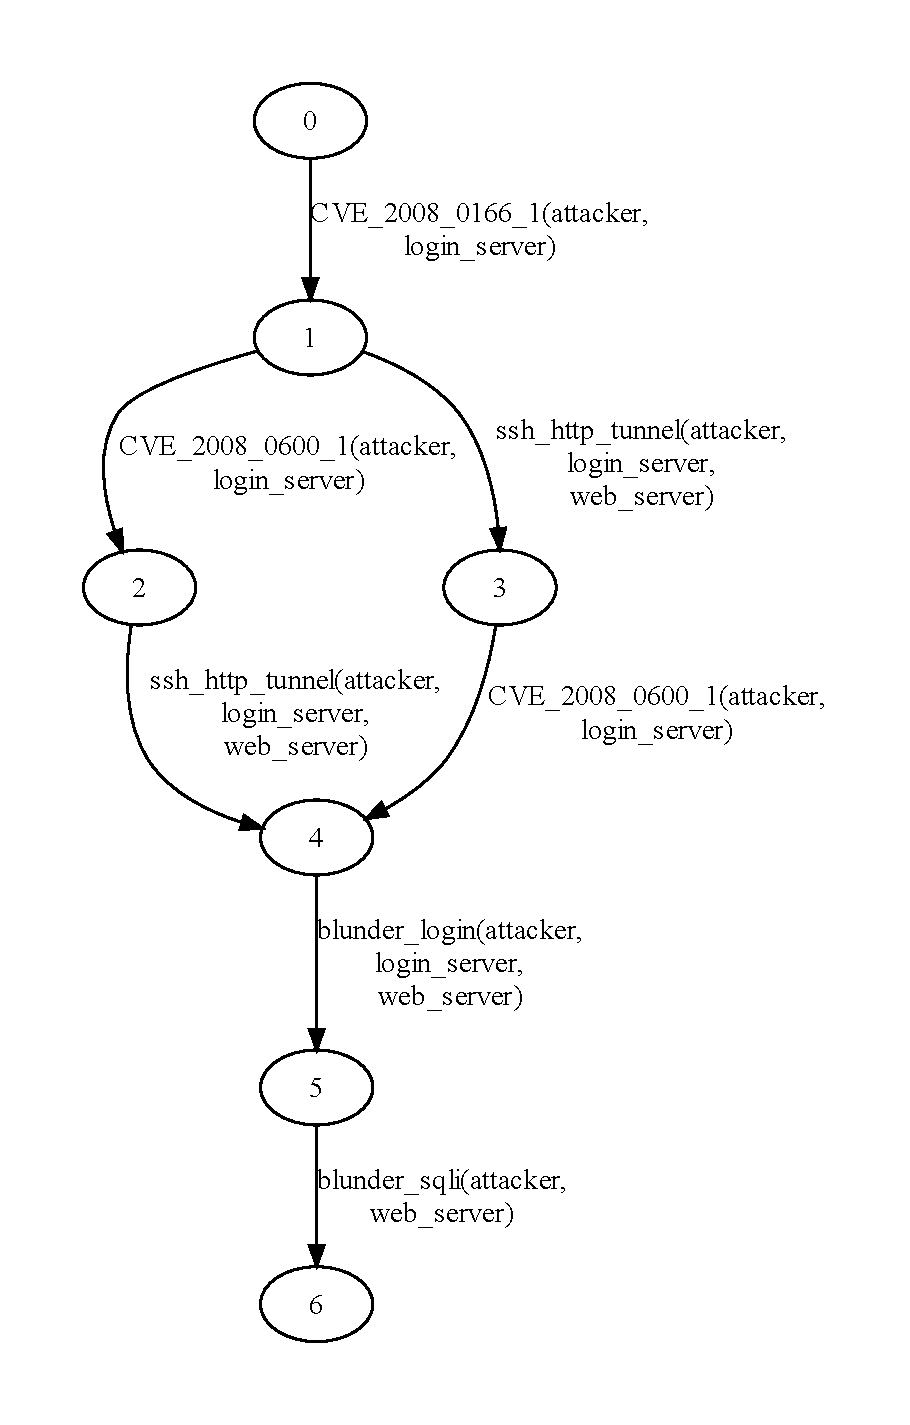
\includegraphics[width=5in]{ag_blunderdome/ag_depth5}
\caption{Blunderdome exercise attack graph}
\label{fig:blunder_ag}
\end{figure}

\begin{figure}
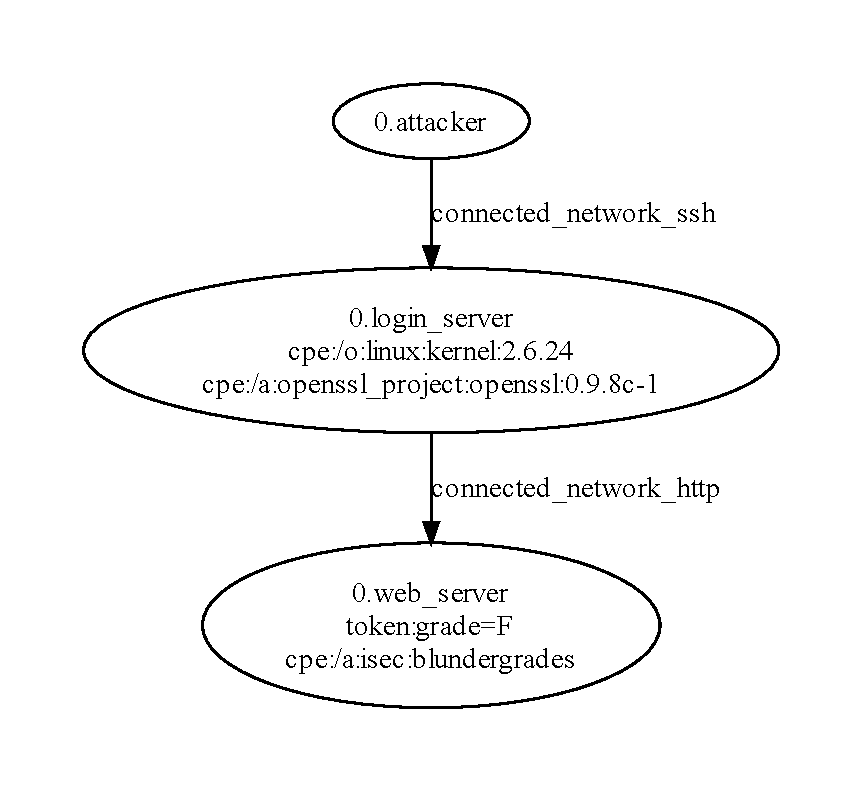
\includegraphics[width=5in]{ag_blunderdome/nm_state0}
\caption{Blunderdome exercise starting state}
\label{fig:blunder_s0}
\end{figure}

\begin{figure}
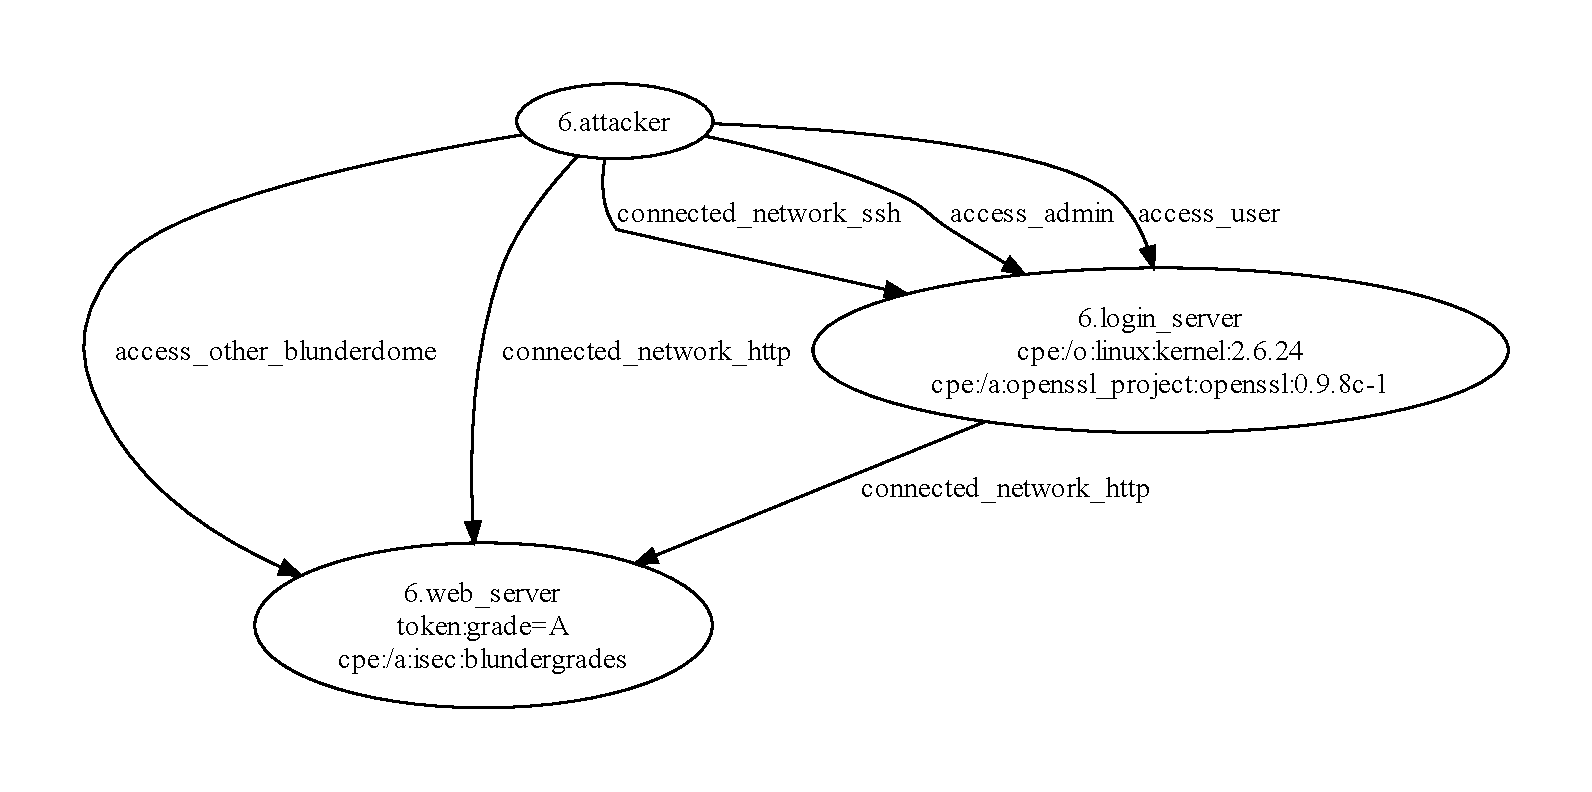
\includegraphics[width=5in]{ag_blunderdome/nm_state6}
\caption{Blunderdome exercise ending state}
\label{fig:blunder_s6}
\end{figure}
